\subsection{SV1}
\label{subsec:sv1}

\def\figpath{figures/ftag/ANA-FTAG-2019-07-PAPER/sv1}

\textbf{Philosophy:} 

SV1 is a vertexing algorithm that reconstructs displaced decays where the set of tracks come from a single secodary vertex.
Although strictly speakig this will rarely be 

Set of input tracks (preselection):
\begin{itemize}
	\item Track cuts: $|d_0| < 3.5\mathrm{mm}$, $|z_0 \sin \theta| < 5\mathrm{mm}$ \cite{giacinto-thesis} and $\pt > 500$~MeVs.
	\item Some track cleaning cuts for jets with $\eta > 1.5$ (since these tracks pass through more material).
	\item Also - only take the 25 highest \pt tracks inside of the jet (helped for reducing the reconstruction of vertices from a random crossing of tracks at high jet \pt \cite[ATL-PHYS-PUB-2017-011].   
\end{itemize}

These track pre-selection cuts are looser than the IPXD (and RIP) algorithms because the next step of selecting the tracks originating from the same point in space acts as another cut on the input tracks. The track \ldots



\begin{itemize}
	\item Form all pairs of 2-track vertices satisfying \cite{giacinto-thesis}:
	\begin{enumerate}
		\item Prob$(\chi^2_{2-trk vtx}) > 3.5$\%
		\item Each track needs to be displaced from the PV with a significance $L_{3D} / \sigma(L_{3D}) > 2\sigma$ and the sum of the two-track significances larger than 6.\footnote{$L_{3D}$ is the 3d distance from the tracks POCA to the PV.}
		\item These tracks need to be ``downstream'' of the jet axis ($\left( \vec{r}_{2 trk} - \vec{r}_{primary} \right) \cdot \vec{p}_{jet} $) \hl{What is $\vec{r}_primary$?}
	\end{enumerate}
	\item Veto tracks that form 2-track vertices consistent with\footnote{The tracker only measures the momentum of the particle, so to reconstruct a mass, we need to make an assumption for what the particle ID is for the mass of the track to get the 4-vector. The meson (or lepton) mass used for each track to reconstruct the 2-track vertex invariant mass is denoted by the subscripts. \hl{I took these numbers from the JF pub note, will need to confirm is they are the same for SV1.}}:
	\begin{enumerate}
		\item $K_s$ decays ( $|m_{\pi^+ \pi^-} - m_{K^0}| < 18$~MeV )
		\item $\lambda$ decays ( $|m_{p \pi^-} - m_{K^0}| < 18$~MeV )
		\item $\gamma$ conversions ($m_{ee} < 30$~MeV)  
		\item hadronic material interactions (veto vertex interactions that overlap with detector material)
	\end{enumerate}
	\item Iterate over this ``cleaned'' set of tracks fitting a single SV  
	\begin{itemize}
		\item If this vertex fix has a $\mathrm{Prob}(\chi^2_{vtx}) < 0.1\%$ -- or -- a vertex mass larger than 6~GeV, remove the track with the largest $\chi^2$ contribution and rise and repeat the fit.
	\end{itemize}	
\end{itemize}


For a true displaced decay, this secondary vertex will have properties consistent with a $B$ or $D$ hadron decay, and some key discriminating variables include the mass of the secondary vertex, the energy fraction, \hl{\ldots}

 \begin{figure}[htbp]
        \centering
        \subfloat[]{ 
                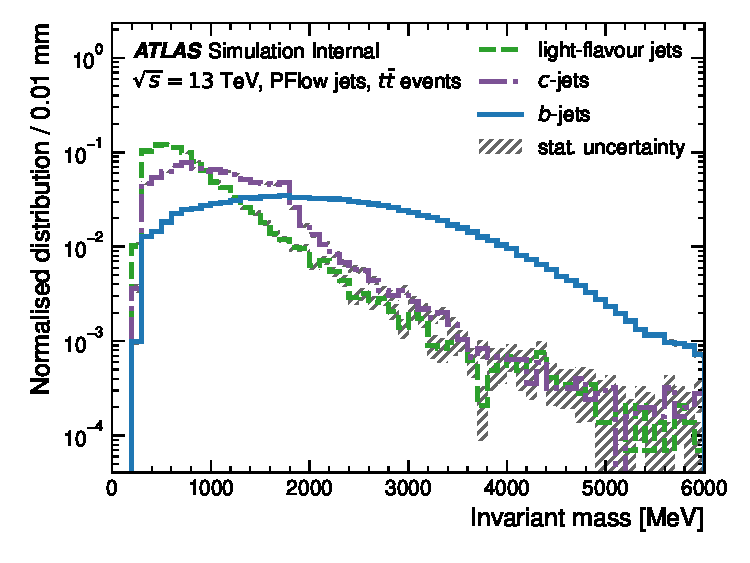
\includegraphics[width=0.32\linewidth]{\figpath/SV1_masssvx_ttbar}
        } 
         \subfloat[]{ 
                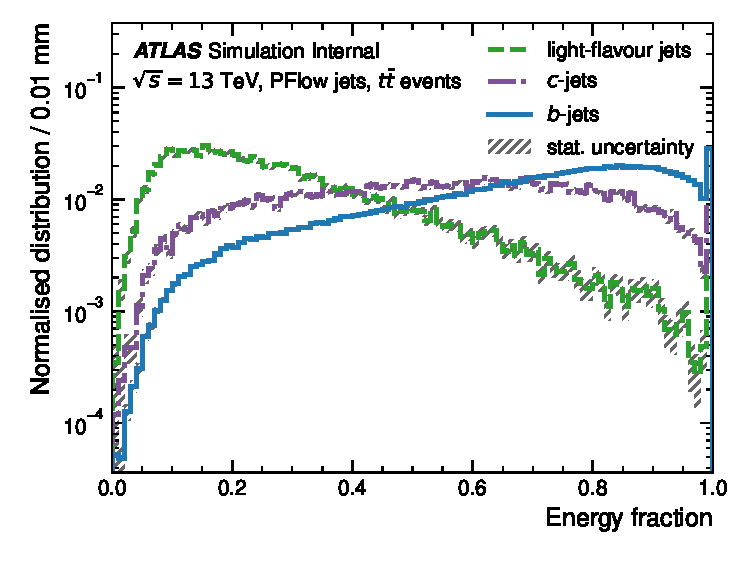
\includegraphics[width=0.32\linewidth]{\figpath/SV1_efracsvx_ttbar.pdf}
        } 
                 \subfloat[]{ 
                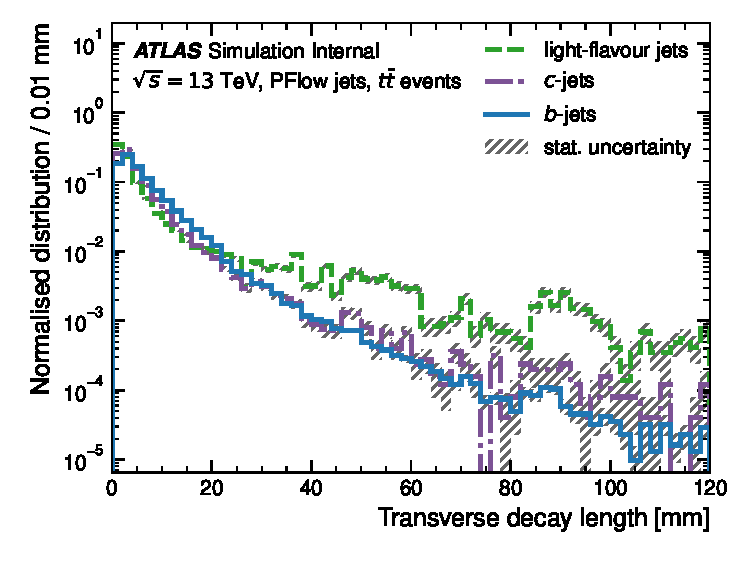
\includegraphics[width=0.32\linewidth]{\figpath/SV1_Lxy_ttbar.pdf}
        } \\ 
        \subfloat[]{ 
                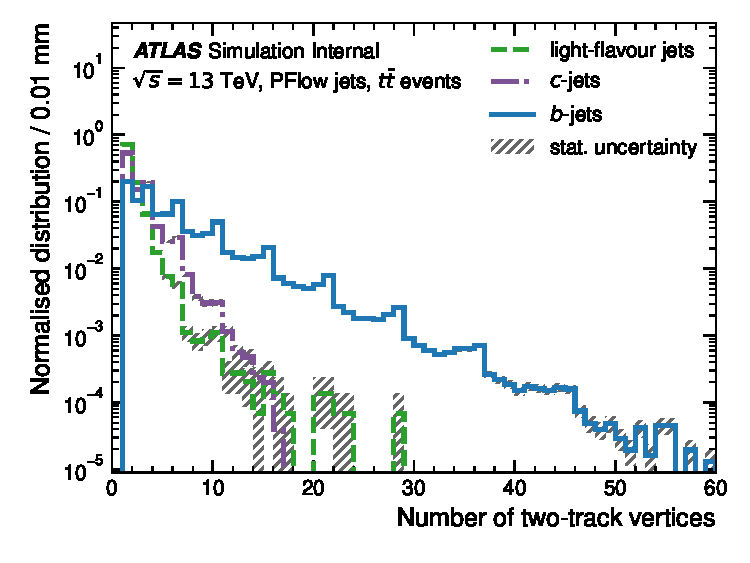
\includegraphics[width=0.32\linewidth]{\figpath/SV1_N2Tpair_ttbar.pdf}
        } 
         \subfloat[]{ 
                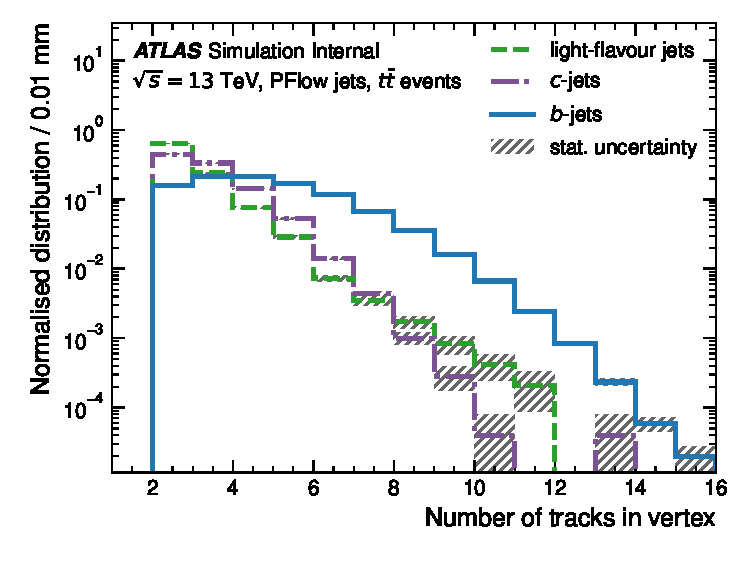
\includegraphics[width=0.32\linewidth]{\figpath/SV1_NGTinSvx_ttbar.pdf}
        } 
                 \subfloat[]{ 
                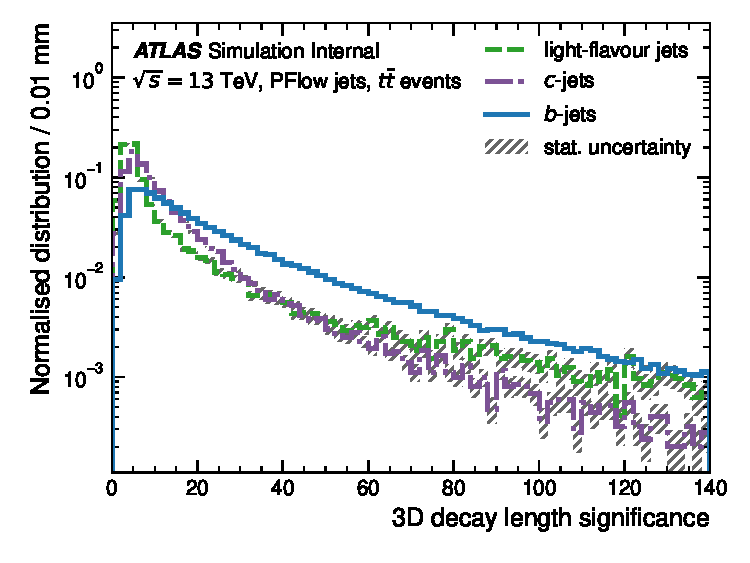
\includegraphics[width=0.32\linewidth]{\figpath/SV1_significance3d_ttbar.pdf}
        } 
        \caption{The SV1 inputs that (will be) in the FTAG algos paper \cite{ANA-FTAG-2019-07}.}
        \label{fig:sv1 inputs}
\end{figure}


\begin{table}[h!]
  \centering
    \begin{tabular}{p{2cm} | p{12cm}  }  
      \textbf{Input} & \textbf{Description}  \\
      \hline
      \hline
  	 $m$ & Invariant mass of the tracks reconstructed in the secondary vertex \\
	 $f_E$ &The energy of the SV over the energy of the jet \\
	 $\Delta R(\vec{p}_{jet},\vec{r_{SV}} - \vec{r_{PV}})$ & Opening angle between the jet and the SV flight axis \\
	 $L_{xy}$ & SV transverse distance from the PV \\
	 $L_{xyz}$ & SV distance from the PV \\
 	 $S_{xyz}$ & Significance of the displacement of the SV: $L_{xyz} / \sigma_{xyz}$ \\
	$n_{vtx \ trk}$ & Number of tracks in the SV \\
	$n_{2-trk vtx}$ & Number of 2 track vertices before the vertex fit \\
    \end{tabular}
    \caption{Features from the SV1 reconstruction that are fed as input to the DL1r tagger.}
    \label{table:jf-inputs}
\end{table}

